To investigate, at least visually, whether the gas mixture reaches equilibrium we plot the time evolution of the averages of the energy of each species. In addition, we include two similar cases with the restitution parameter $\xi$ set to $0.9$ and $0.8$. This is shown in figure \ref{fig:averages}. By the very definition of thermal equilibrium, e.g. the one given in \cite[p.~3]{huang}

\begin{displayquote}
	Thermodynamic equilibrium prevails when the thermodynamic state of
	the system does not change with time.
\end{displayquote}
	
it is clear that the system cannot reach equilibrium in the presence of energy dissipation.

The plot in figure \ref{fig:averages} shows that the two different particle species reach equilibrium only in the case where the energy is conserved. Furthermore, it is seen that the heavy gas molecules are always at higher temperature in the two latter cases. Although this fact is easily realised from elementary statistical mechanics, demonstrating it through these simulations is a good check that the correct physics is contained within the model made. 

\begin{figure}[htb]
	\centering
	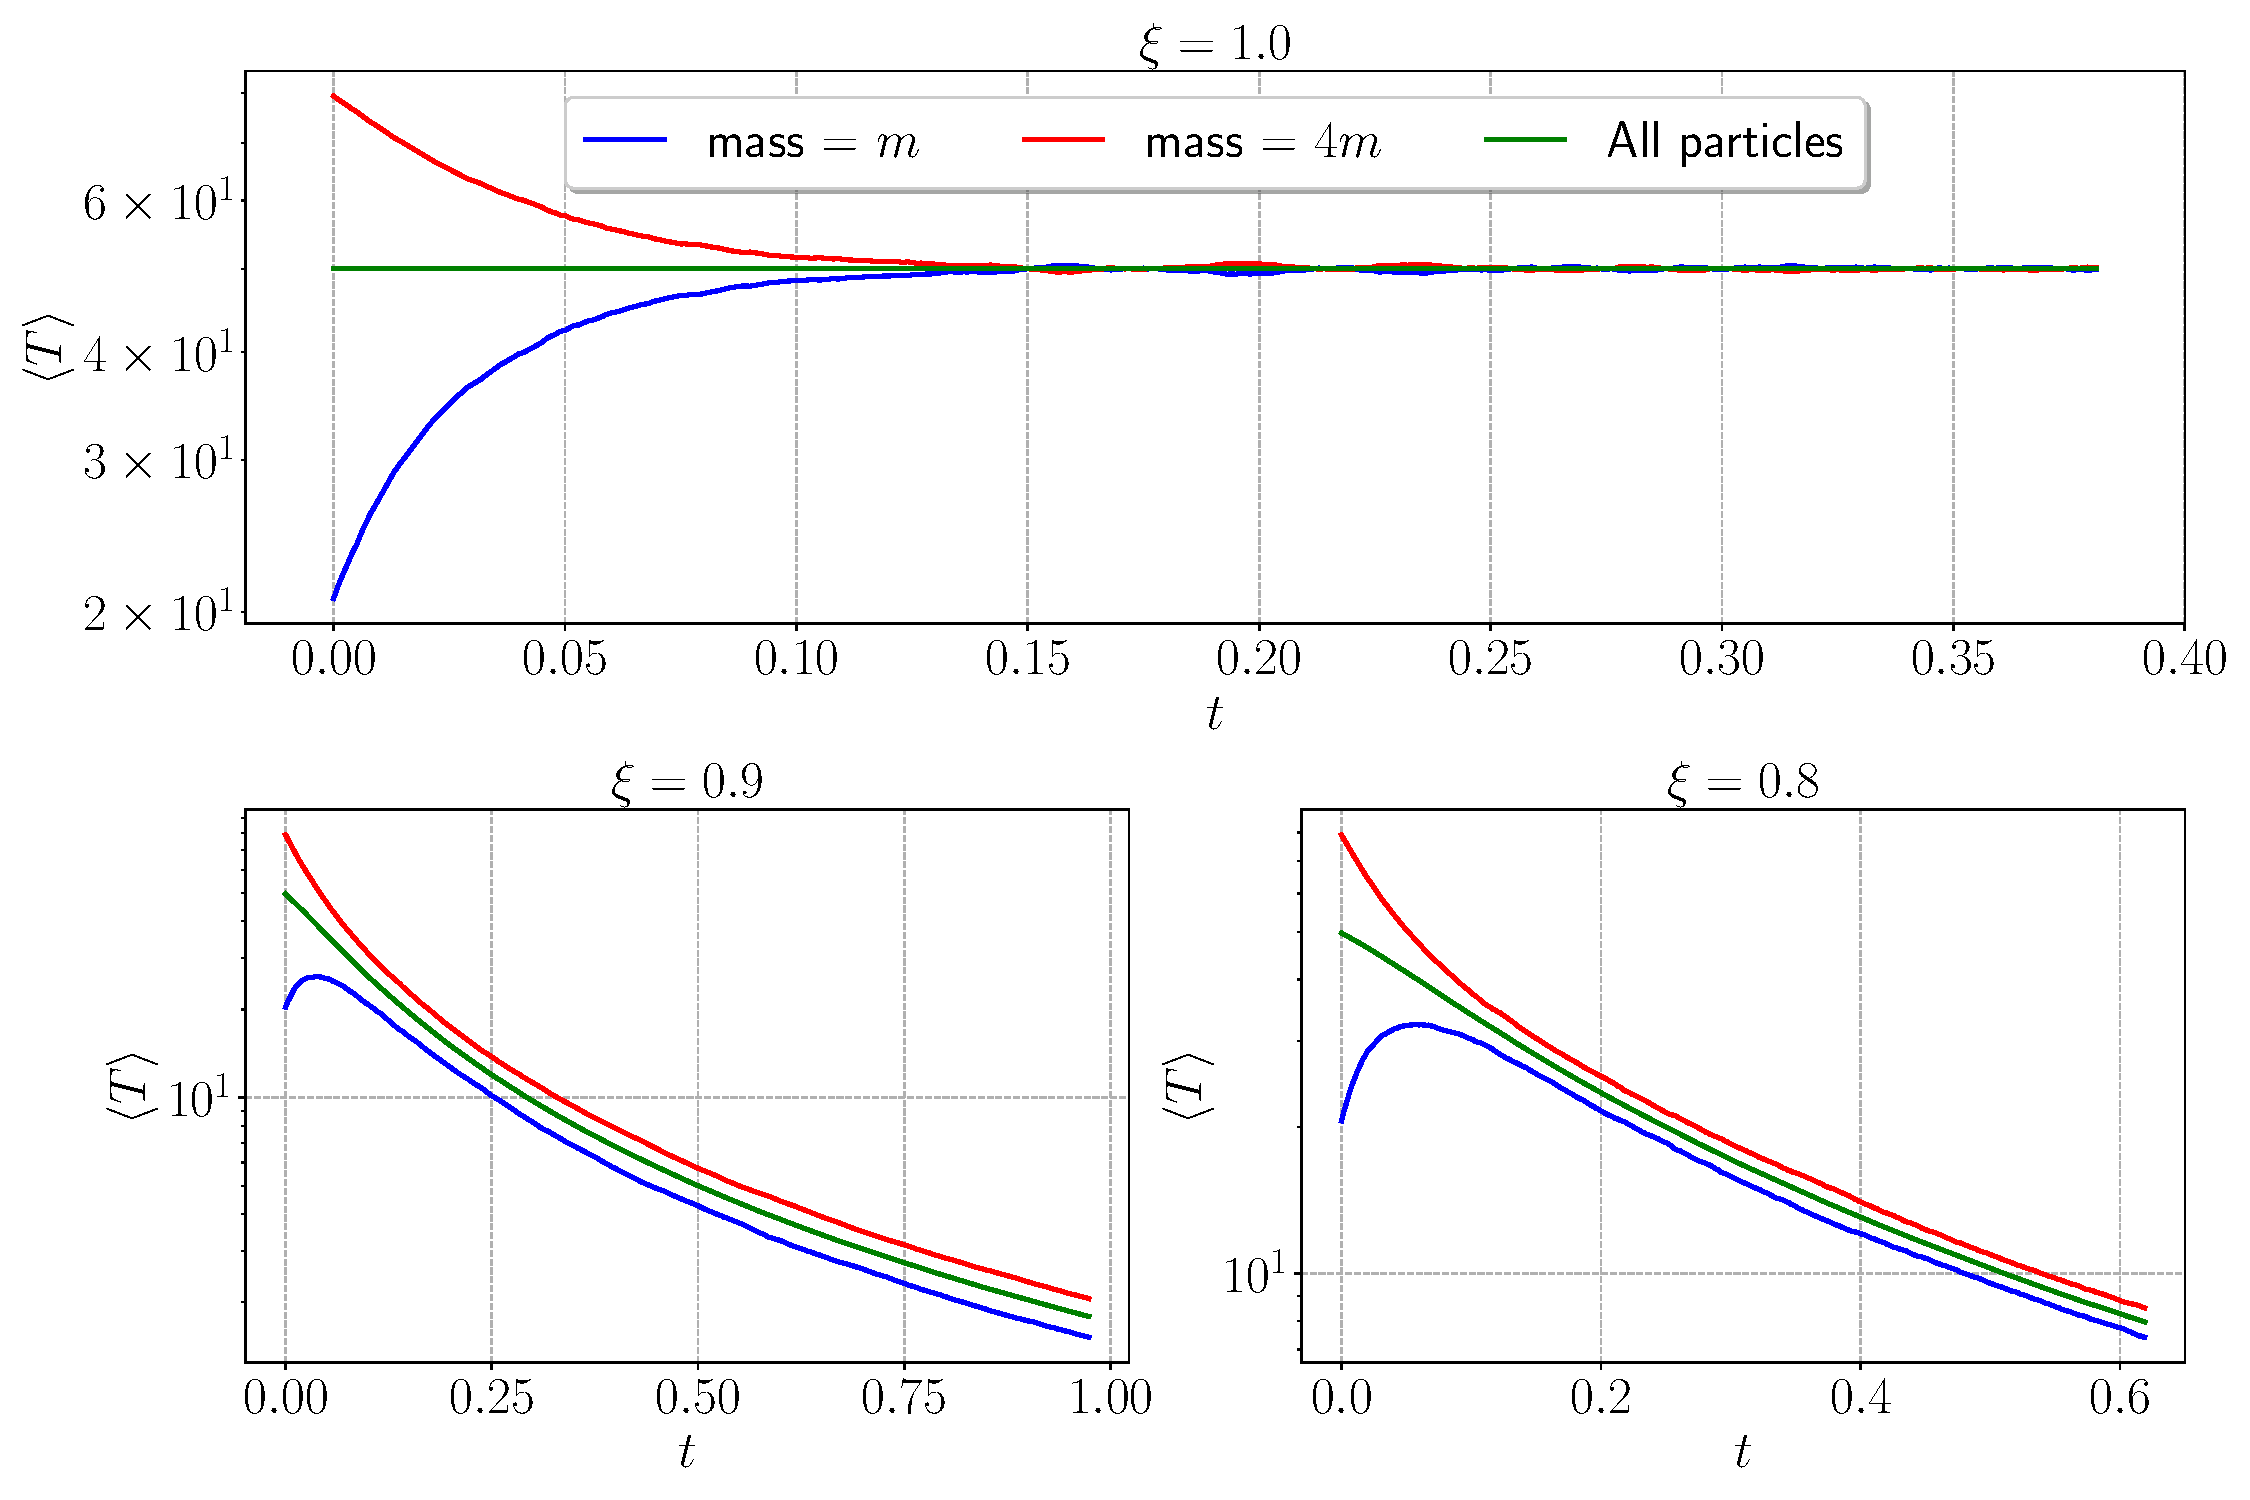
\includegraphics[width = \columnwidth]{../fig/energy_avg.pdf}
	\caption{Time evolution of energy averages for restitution parameter $\xi = 1.0,0.9,0.8$. The data comes from an ensemble of $8$ gases with $4000$ particles each.}
	\label{fig:averages}
\end{figure}

